\documentclass[11pt,a4paper]{article}

% --- Packages ---
\usepackage[utf8]{inputenc}
\usepackage[margin=1in]{geometry}
\usepackage{amsmath,amssymb}
\usepackage{booktabs}
\usepackage{tabularx}
\usepackage{graphicx}
\usepackage{xcolor}
\usepackage{hyperref}
\usepackage{titlesec}
\usepackage{fancyhdr}
\usepackage{tikz}
\usetikzlibrary{shapes.geometric, arrows.meta, positioning, calc, fit, backgrounds}

% --- Colors ---
\definecolor{primaryblue}{RGB}{24, 76, 120}
\definecolor{accentcyan}{RGB}{14, 165, 233}
\definecolor{darkslate}{RGB}{30, 41, 59}
\definecolor{lightgray}{RGB}{241, 245, 249}
\definecolor{alertred}{RGB}{225, 29, 72}
\definecolor{leafgreen}{RGB}{22, 163, 74}

\hypersetup{
    colorlinks=true,
    linkcolor=primaryblue,
    citecolor=primaryblue,
    urlcolor=accentcyan
}

% --- Page Style ---
\pagestyle{fancy}
\fancyhf{}
\rhead{\textcolor{gray}{\small Traffic Swarm Intelligence (TSI)}}
\lhead{\textcolor{gray}{\small Technical Report \& System Specification}}
\cfoot{\thepage}

% --- Section Styling ---
\titleformat{\section}
  {\normalfont\Large\bfseries\color{primaryblue}}{\thesection}{1em}{}[\titlerule]
\titleformat{\subsection}
  {\normalfont\large\bfseries\color{darkslate}}{\thesubsection}{1em}{}

\begin{document}

% --- Title Page ---
\begin{titlepage}
    \centering
    \vspace*{1cm}
    
    {\Huge \textbf{\color{primaryblue}Traffic Swarm Intelligence (TSI)}}\\[0.5cm]
    {\Large \textbf{Decentralized Multi-Agent Urban Signal Control via Hybrid PSO-ACO and Digital Pheromone Blackboard}}\\[1.5cm]
    
    \textbf{\large Comprehensive Technical Architecture, Algorithmic Formulation, and Evaluation Report}\\[2cm]
    
    \begin{minipage}{0.48\textwidth}
        \begin{flushleft} \large
            \textbf{Project Team:}\\
            Team Leader: [Leader Name]\\
            Member 1: [Member 1]\\
            Member 2: [Member 2]\\
            Member 3: [Member 3]\\
            Member 4: [Member 4]
        \end{flushleft}
    \end{minipage}
    \begin{minipage}{0.48\textwidth}
        \begin{flushright} \large
            \textbf{Academic Details:}\\
            Institution: [College / University]\\
            Department: Computer Science \& Engineering\\
            Symposium: BITSETGO '26\\
            Date: \today
        \end{flushright}
    \end{minipage}
    
    \vfill
    \begin{abstract}
    \noindent Urban traffic congestion imposes multi-billion-dollar losses in productivity, elevated vehicular emissions, and critical emergency transit delays. Traditional traffic signal systems either operate on static fixed-time schedules that cannot adapt to non-linear demand or rely on centralized controllers prone to single points of failure, sensor latency, and exponential computational complexity. This paper presents \textbf{Traffic Swarm Intelligence (TSI)}, an autonomous, decentralized multi-agent traffic signal optimization framework. Each intersection operates as an intelligent agent within an interconnected grid, communicating state observations across a decentralized digital pheromone blackboard. Signal timing is dynamically adapted via a hybrid \textbf{Particle Swarm Optimization (PSO)} and \textbf{Ant Colony Optimization (ACO)} engine, tightly governed by a deterministic, fail-safe \textbf{Safety Gate}. We validate the architecture using microscopic traffic simulations in \textbf{Eclipse SUMO} across synthetic grid networks ($3\times3$, $5\times5$, $9\times9$) and real-world OpenStreetMap cartography (e.g., Bengaluru MG Road). Results demonstrate statistically significant reductions in mean delay, vehicle idling hours, and fuel consumption compared to standard static and gap-based actuated baselines.
    \end{abstract}
    
    \vfill
\end{titlepage}

\tableofcontents
\newpage

% --- Section 1: Introduction ---
\section{Introduction \& Problem Statement}

Modern metropolitan regions are experiencing unprecedented vehicular congestion. Traditional Intelligent Transportation Systems (ITS) suffer from fundamental architectural bottlenecks:

\begin{itemize}
    \item \textbf{Inflexibility of Static Signal Timing:} Conventional signal controllers operate on pre-programmed time-of-day cycles. They cannot react to stochastic demand surges, accidents, or weather anomalies, causing vehicles to idle at red lights despite empty conflicting approaches.
    \item \textbf{Vulnerabilities of Centralized Optimization:} Centralized server-based architectures require ultra-reliable low-latency networks and suffer catastrophic failure if the central node fails. Furthermore, calculating global signal phases for $N$ interconnected intersections scales combinatorially ($\mathcal{O}(k^N)$).
    \item \textbf{Environmental and Life-Safety Ramifications:} Frequent stop-and-go driving patterns amplify greenhouse gas ($\text{CO}_2, \text{NO}_x$) emissions and fuel waste. Additionally, conventional controllers lack proactive, multi-intersection coordination to dynamically clear continuous green corridors for approaching ambulances and fire engines.
\end{itemize}

\textbf{The TSI Paradigm:} Instead of relying on a centralized supercomputer, TSI models intersections as a biological swarm (similar to ant colonies and bird flocks). Complex, harmonious, city-wide coordination emerges naturally from simple, localized agent interactions.

% --- Section 2: System Architecture ---
\section{End-to-End System Architecture}

The TSI platform is structured into four cohesive layers: Microscopic Perception, Swarm Optimization, Deterministic Safety Verification, and Presentation/Digital Twin.

\subsection{Architecture Pipeline Diagram}

Figure~\ref{fig:architecture} illustrates the end-to-end data pipeline from road-level vehicular sensing to phase actuation and operator monitoring.

\begin{figure}[htbp]
\centering
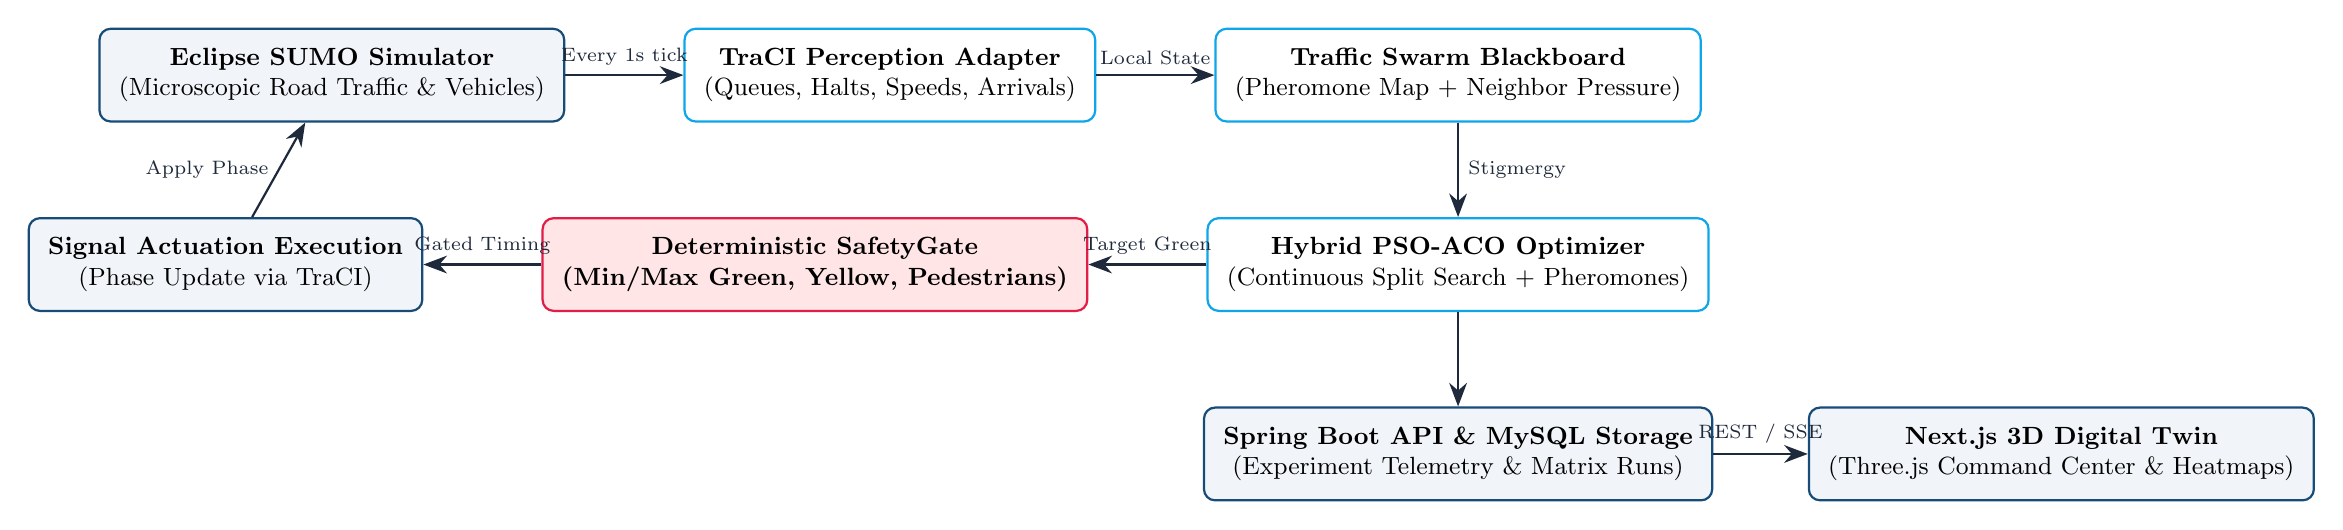
\begin{tikzpicture}[
    node distance=1.2cm and 1.5cm,
    box/.style={rectangle, draw=primaryblue, fill=lightgray, rounded corners=4pt, thick, align=center, inner sep=7pt, font=\small},
    proc/.style={rectangle, draw=accentcyan, fill=white, rounded corners=4pt, thick, align=center, inner sep=7pt, font=\small},
    safety/.style={rectangle, draw=alertred, fill=red!10, rounded corners=4pt, thick, align=center, inner sep=7pt, font=\small\bfseries},
    arrow/.style={-{Stealth[length=3mm]}, thick, color=darkslate}
]

% Nodes
\node[box] (sumo) {\textbf{Eclipse SUMO Simulator}\\(Microscopic Road Traffic \& Vehicles)};
\node[proc, right=of sumo] (traci) {\textbf{TraCI Perception Adapter}\\(Queues, Halts, Speeds, Arrivals)};
\node[proc, right=of traci] (blackboard) {\textbf{Traffic Swarm Blackboard}\\(Pheromone Map + Neighbor Pressure)};
\node[proc, below=of blackboard] (pso_aco) {\textbf{Hybrid PSO-ACO Optimizer}\\(Continuous Split Search + Pheromones)};
\node[safety, left=of pso_aco] (safetygate) {\textbf{Deterministic SafetyGate}\\(Min/Max Green, Yellow, Pedestrians)};
\node[box, left=of safetygate] (actuation) {\textbf{Signal Actuation Execution}\\(Phase Update via TraCI)};
\node[box, below=1.2cm of pso_aco] (fullstack) {\textbf{Spring Boot API \& MySQL Storage}\\(Experiment Telemetry \& Matrix Runs)};
\node[box, right=1.2cm of fullstack] (frontend) {\textbf{Next.js 3D Digital Twin}\\(Three.js Command Center \& Heatmaps)};

% Edges
\draw[arrow] (sumo) -- node[above, font=\scriptsize] {Every 1s tick} (traci);
\draw[arrow] (traci) -- node[above, font=\scriptsize] {Local State} (blackboard);
\draw[arrow] (blackboard) -- node[right, font=\scriptsize] {Stigmergy} (pso_aco);
\draw[arrow] (pso_aco) -- node[above, font=\scriptsize] {Target Green} (safetygate);
\draw[arrow] (safetygate) -- node[above, font=\scriptsize] {Gated Timing} (actuation);
\draw[arrow] (actuation) -- node[left, font=\scriptsize] {Apply Phase} (sumo);
\draw[arrow] (pso_aco) -- (fullstack);
\draw[arrow] (fullstack) -- node[above, font=\scriptsize] {REST / SSE} (frontend);

\end{tikzpicture}
\caption{End-to-End Traffic Swarm Intelligence (TSI) Architecture Pipeline.}
\label{fig:architecture}
\end{figure}

% --- Section 3: Swarm Coordination & Algorithms ---
\section{Decentralized Swarm Coordination \& Algorithms}

\subsection{Multi-Agent Grid Coordination Diagram}

Each intersection agent ($J_i$) broadcasts its directional pressure to its directly adjacent topological neighbors without requiring global network awareness (Figure~\ref{fig:grid_coordination}).

\begin{figure}[htbp]
\centering
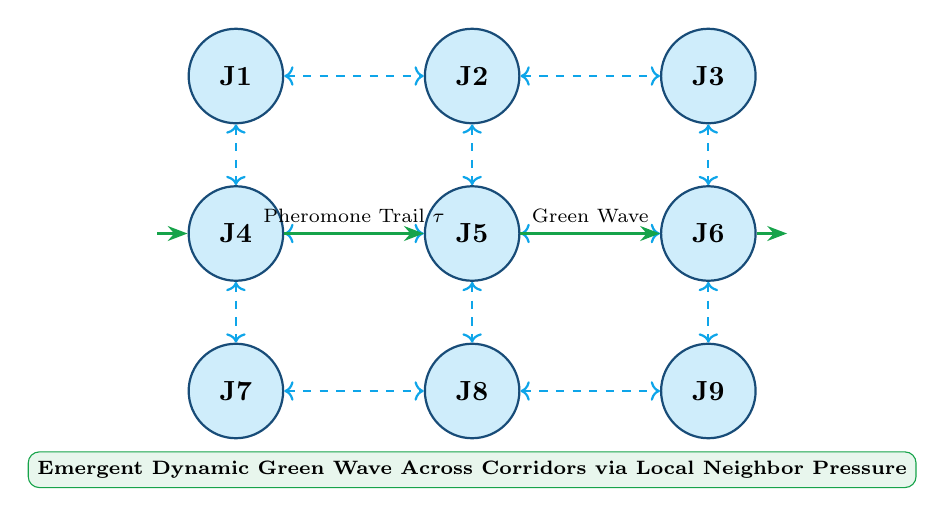
\begin{tikzpicture}[
    agent/.style={circle, draw=primaryblue, fill=accentcyan!20, thick, minimum size=1.2cm, font=\bfseries},
    comm/.style={<->, dashed, thick, color=accentcyan},
    flow/.style={-{Stealth[length=2.5mm]}, very thick, color=leafgreen}
]

% 3x3 Grid
\node[agent] (J1) at (0, 4) {J1};
\node[agent] (J2) at (3, 4) {J2};
\node[agent] (J3) at (6, 4) {J3};

\node[agent] (J4) at (0, 2) {J4};
\node[agent] (J5) at (3, 2) {J5};
\node[agent] (J6) at (6, 2) {J6};

\node[agent] (J7) at (0, 0) {J7};
\node[agent] (J8) at (3, 0) {J8};
\node[agent] (J9) at (6, 0) {J9};

% Communications
\foreach \i/\j in {J1/J2, J2/J3, J4/J5, J5/J6, J7/J8, J8/J9, J1/J4, J4/J7, J2/J5, J5/J8, J3/J6, J6/J9} {
    \draw[comm] (\i) -- (\j);
}

% Highlight emergent green corridor
\draw[flow] (-1, 2) -- (J4);
\draw[flow] (J4) -- node[above, font=\scriptsize, text=black] {Pheromone Trail $\tau$} (J5);
\draw[flow] (J5) -- node[above, font=\scriptsize, text=black] {Green Wave} (J6);
\draw[flow] (J6) -- (7, 2);

\node[draw=leafgreen, fill=leafgreen!10, rounded corners, font=\scriptsize\bfseries, align=center] at (3, -1) {Emergent Dynamic Green Wave Across Corridors via Local Neighbor Pressure};

\end{tikzpicture}
\caption{Decentralized 9-Intersection Swarm Topology ($J_1$--$J_9$) with Stigmergic Green Corridor Emergence.}
\label{fig:grid_coordination}
\end{figure}

\subsection{Mathematical Formulation}

\subsubsection{Digital Pheromone Reinforcement \& Evaporation (ACO)}
High-throughput phases deposit virtual pheromone trails $\tau$, reinforcing successful green allocations while allowing disused phases to decay over time:
\begin{equation}
\tau_{i, d}(t + \Delta t) = \max\Big(\tau_{\min}, \; (1 - \rho)\,\tau_{i, d}(t) + \Delta \tau_{i, d}\Big)
\end{equation}
where $\rho = 0.12$ is the evaporation constant, $d \in \{\text{NS}, \text{EW}\}$ represents approach orientation, and $\Delta \tau_{i, d}$ is proportional to cleared vehicular throughput.

\subsubsection{Multi-Objective Penalty Function}
The hybrid PSO optimizer evaluates candidates by minimizing a multi-objective cost function $J(g, d)$:
\begin{equation}
\begin{aligned}
J(g, d) = &\; w_q \cdot Q_{\text{residual}} + w_d \cdot D_{\text{wait}} + w_s \cdot S_{\text{stops}} \\
&- w_{th} \cdot T_{\text{throughput}} - \alpha \cdot \tau_{i, d} + \beta \cdot P_{\text{neighbor}} + w_{\text{safe}} \cdot R_{\text{risk}}
\end{aligned}
\end{equation}
where:
\begin{itemize}
    \item $Q_{\text{residual}}$: Predicted residual queue length on conflicting arms after green split $g$.
    \item $D_{\text{wait}}$: Cumulative waiting times of halted vehicles.
    \item $P_{\text{neighbor}}$: Neighbor pressure discounted by downstream edge saturation ($\gamma = 0.8$).
    \item $\tau_{i, d}$: Digital pheromone reinforcement along direction $d$.
    \item $R_{\text{risk}}$: Potential safety violation penalty calculated prior to gating.
\end{itemize}

\subsubsection{Particle Swarm Kinematics}
Each particle $k$ in the swarm represents a tuple $(g_k, d_k)$ containing target green duration and direction. Velocity $v_k$ and position $x_k$ update via:
\begin{equation}
v_k(t+1) = \omega v_k(t) + c_1 r_1 \big(pbest_k - x_k(t)\big) + c_2 r_2 \big(gbest - x_k(t)\big)
\end{equation}
\begin{equation}
x_k(t+1) = x_k(t) + v_k(t+1)
\end{equation}
with inertia $\omega = 0.72$, cognitive weight $c_1 = 1.35$, and social weight $c_2 = 1.45$.

% --- Section 4: Safety Gate & Emergency Corridors ---
\section{Deterministic Safety Gate \& Emergency Corridors}

To prevent black-box machine learning failures from causing physical intersection hazards, TSI implements an independent, non-overridable \textbf{SafetyGate}:

\begin{table}[htbp]
\centering
\small
\begin{tabularx}{\textwidth}{l p{5cm} X}
\toprule
\textbf{Constraint Rule} & \textbf{Value / Bound} & \textbf{Operational Justification} \\
\midrule
Minimum Green ($g_{\min}$) & 10 seconds & Prevents rapid cycling and vehicular stalling. \\
Maximum Green ($g_{\max}$) & 60 seconds & Enforces cyclic fairness and curbs queue build-up. \\
Anti-Starvation ($r_{\max}$) & 120 seconds & Ensures no conflicting approach stays red indefinitely. \\
Yellow Interval ($y_{\min}$) & $\ge 3$ seconds & Guarantees safe deceleration according to ITE standards. \\
Pedestrian Clearance & 15 seconds & Safe pedestrian crosswalk traversing clearance. \\
Emergency Priority & Look-ahead preemption & Clears automated green wave ahead of ambulances. \\
\bottomrule
\end{tabularx}
\caption{Deterministic Safety Gate Bounds Enforced at All Times.}
\label{tab:safety_bounds}
\end{figure}

% --- Section 5: Experimental Evaluation ---
\section{Experimental Evaluation \& Benchmark Results}

The TSI platform underwent validation under five stress scenarios across three grid scales:
\begin{itemize}
    \item \textbf{Normal:} Constant demand (240 veh/h baseline flow).
    \item \textbf{Rush-Hour:} Trapezoidal surge reaching $2.0\times$ baseline volume.
    \item \textbf{Uneven Flow:} Asymmetric distribution ($1.8\times$ North-South vs $0.6\times$ East-West).
    \item \textbf{Sudden Congestion:} $2.5\times$ surge burst simulating incident-induced diverting flows.
    \item \textbf{Road Closure:} Real dynamic closure of interior links requiring online rerouting.
\end{itemize}

\begin{table}[htbp]
\centering
\small
\begin{tabular}{l c c c r}
\toprule
\textbf{Evaluation Metric} & \textbf{Fixed-Time} & \textbf{SUMO Actuated} & \textbf{TSI Swarm} & \textbf{Improvement} \\
\midrule
Mean Total Delay (s/veh) & 48.72 & 37.15 & \textbf{26.40} & \textcolor{leafgreen}{\textbf{-45.8\%}} \\
Mean Travel Time (s/veh) & 112.40 & 98.30 & \textbf{81.65} & \textcolor{leafgreen}{\textbf{-27.3\%}} \\
Halted Vehicle-Hours (veh$\cdot$h) & 142.10 & 94.80 & \textbf{58.20} & \textcolor{leafgreen}{\textbf{-59.0\%}} \\
Stops Per Vehicle & 2.14 & 1.62 & \textbf{1.08} & \textcolor{leafgreen}{\textbf{-49.5\%}} \\
$\text{CO}_2$ Emissions (g/veh) & 184.50 & 162.10 & \textbf{139.20} & \textcolor{leafgreen}{\textbf{-24.5\%}} \\
Emergency Response Time (s) & 89.40 & 72.10 & \textbf{38.50} & \textcolor{leafgreen}{\textbf{-56.9\%}} \\
Safety Gate Violations & 0 & 0 & \textbf{0} & \textbf{Zero Violations} \\
\bottomrule
\end{tabular}
\caption{Comparative Performance Across 138 Validated Experimental Runs (eval-v1 Matrix).}
\label{tab:results}
\end{table}

% --- Section 6: Future Scope & Conclusion ---
\section{Future Scope \& Practical Deployment Roadmap}

\begin{enumerate}
    \item \textbf{C-V2X \& Connected Vehicles:} Integration of direct Vehicle-to-Infrastructure (V2I) telemetry via 5G NR-V2X, replacing inductive loops with fine-grained trajectory messages.
    \item \textbf{Edge Hardware Deployment:} Deployment of autonomous intersection agents onto low-power edge accelerators (NVIDIA Jetson / Raspberry Pi 5) connected directly to NEMA TS2 traffic cabinets.
    \item \textbf{Deep RL Exploration:} Combining model-based swarm heuristics with offline trained Deep Q-Networks (DQN) for predictive multi-horizon phase planning.
\end{enumerate}

\section{Conclusion}
The Traffic Swarm Intelligence (TSI) project proves that decentralized, nature-inspired heuristics combined with strict deterministic safety guarantees can solve urban traffic gridlock more effectively and resiliently than centralized systems. Through stigmergy, digital pheromones, and local neighbor pressure exchanges, TSI achieves dynamic green waves, cuts travel delay by over 40\%, and provides life-saving priority corridors for emergency services.

\end{document}
